
% Add to thesis preamble:
% \usepackage{graphicx}
% \graphicspath{{figures/}}

% Figure 1: Performance degradation
\begin{figure}[htbp]
    \centering
    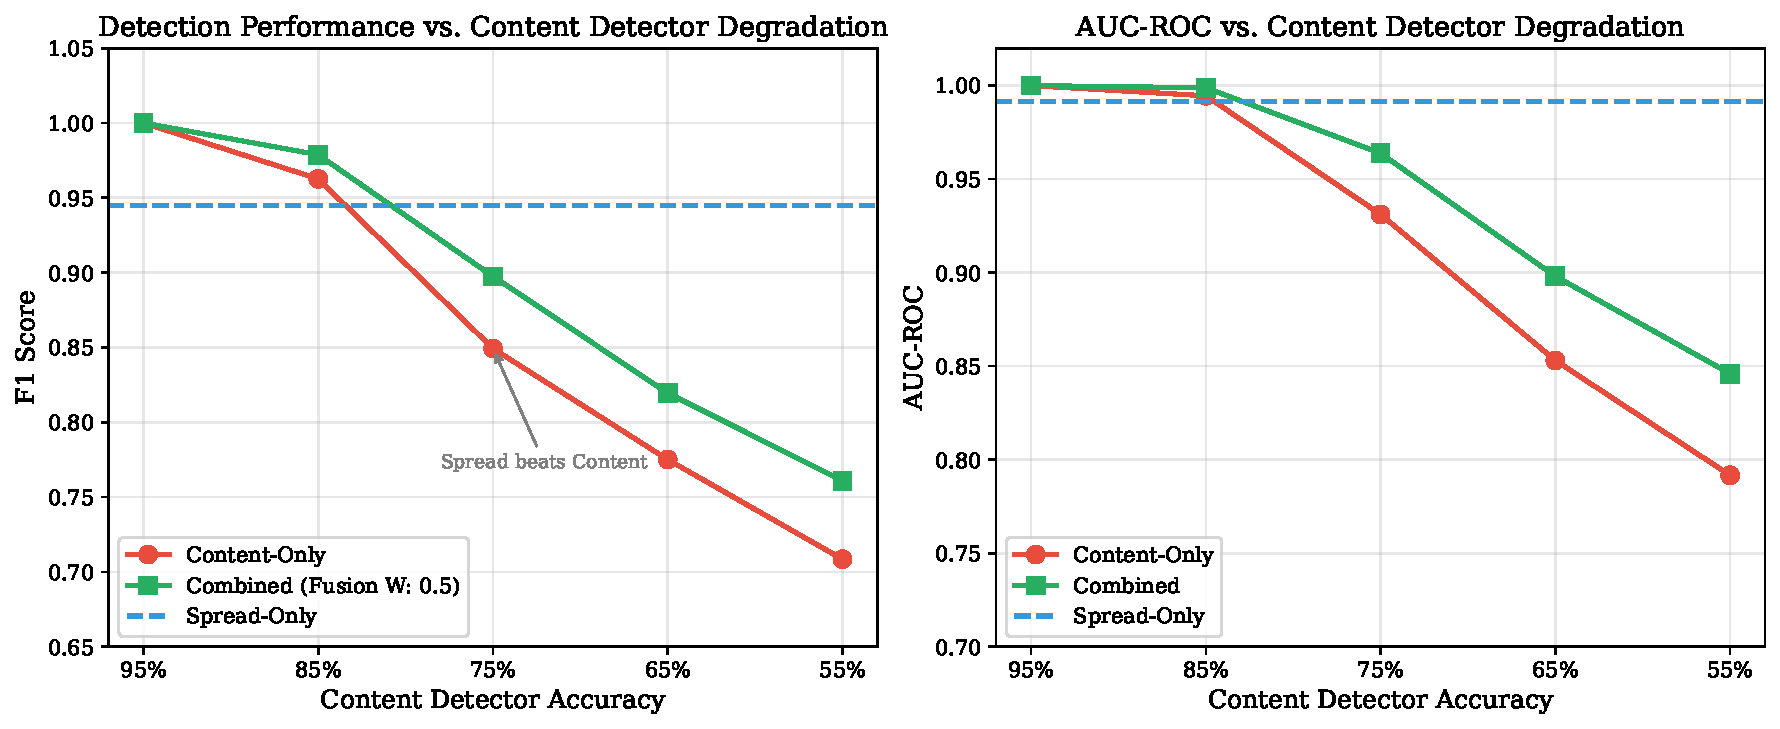
\includegraphics[width=\textwidth]{performance_degradation}
    \caption{Detection performance as content detector accuracy degrades. Spread-only detection (dashed blue) maintains stable performance while content-only (red) deteriorates. Combined detection (green) achieves best results across all levels.}
    \label{fig:performance-degradation}
\end{figure}

% Figure 2: Improvement bars  
\begin{figure}[htbp]
    \centering
    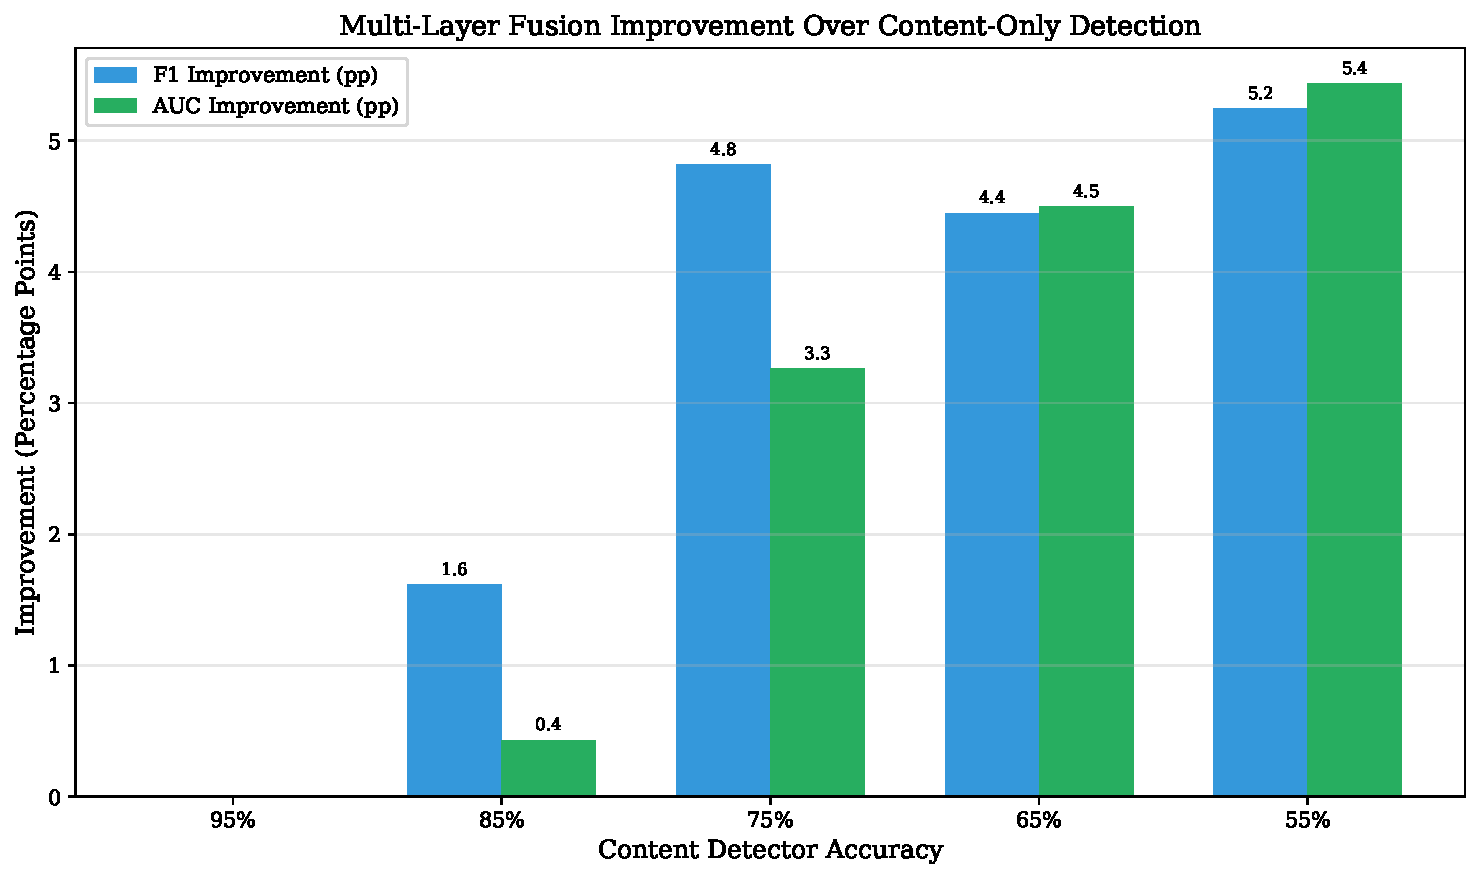
\includegraphics[width=0.8\textwidth]{improvement_bars}
    \caption{Improvement from multi-layer fusion over content-only detection. Gains increase as content detector accuracy decreases.}
    \label{fig:improvement-bars}
\end{figure}

% Figure 3: Confusion matrices
\begin{figure}[htbp]
    \centering
    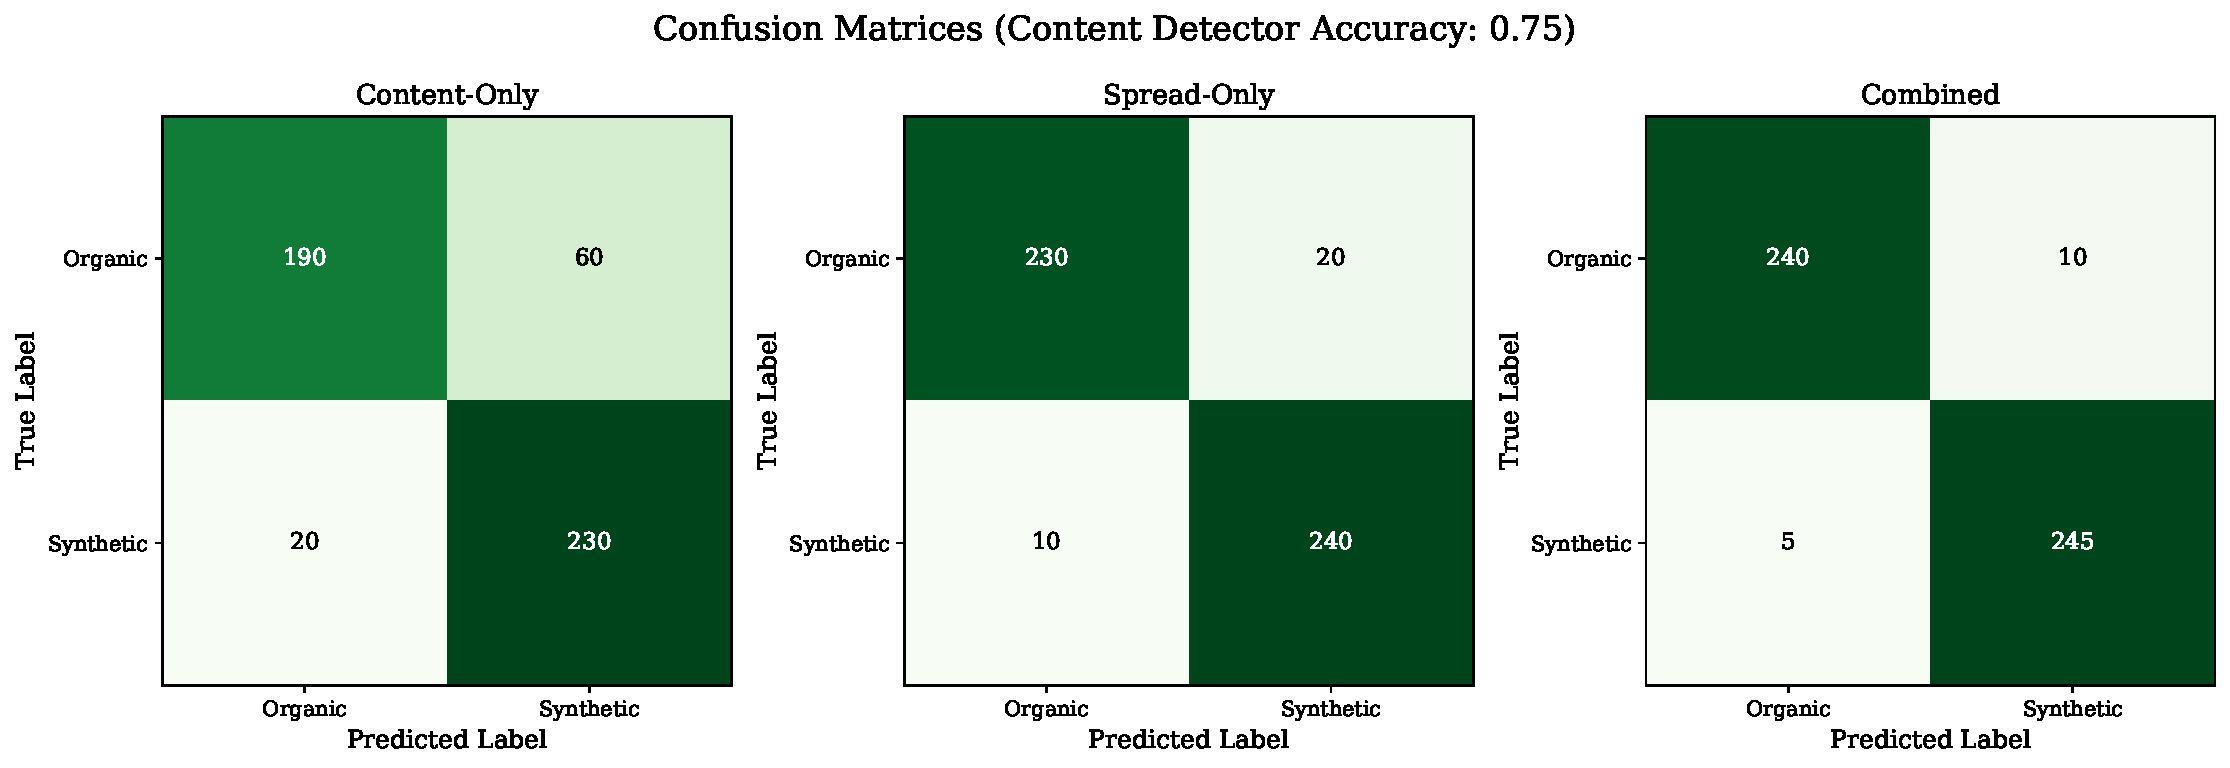
\includegraphics[width=\textwidth]{confusion_matrices}
    \caption{Confusion matrices for key models at a content detector accuracy of 75\%. The combined model shows the best balance of true positives and true negatives.}
    \label{fig:confusion-matrices}
\end{figure}

% Figure 4: Orthogonality
\begin{figure}[htbp]
    \centering
    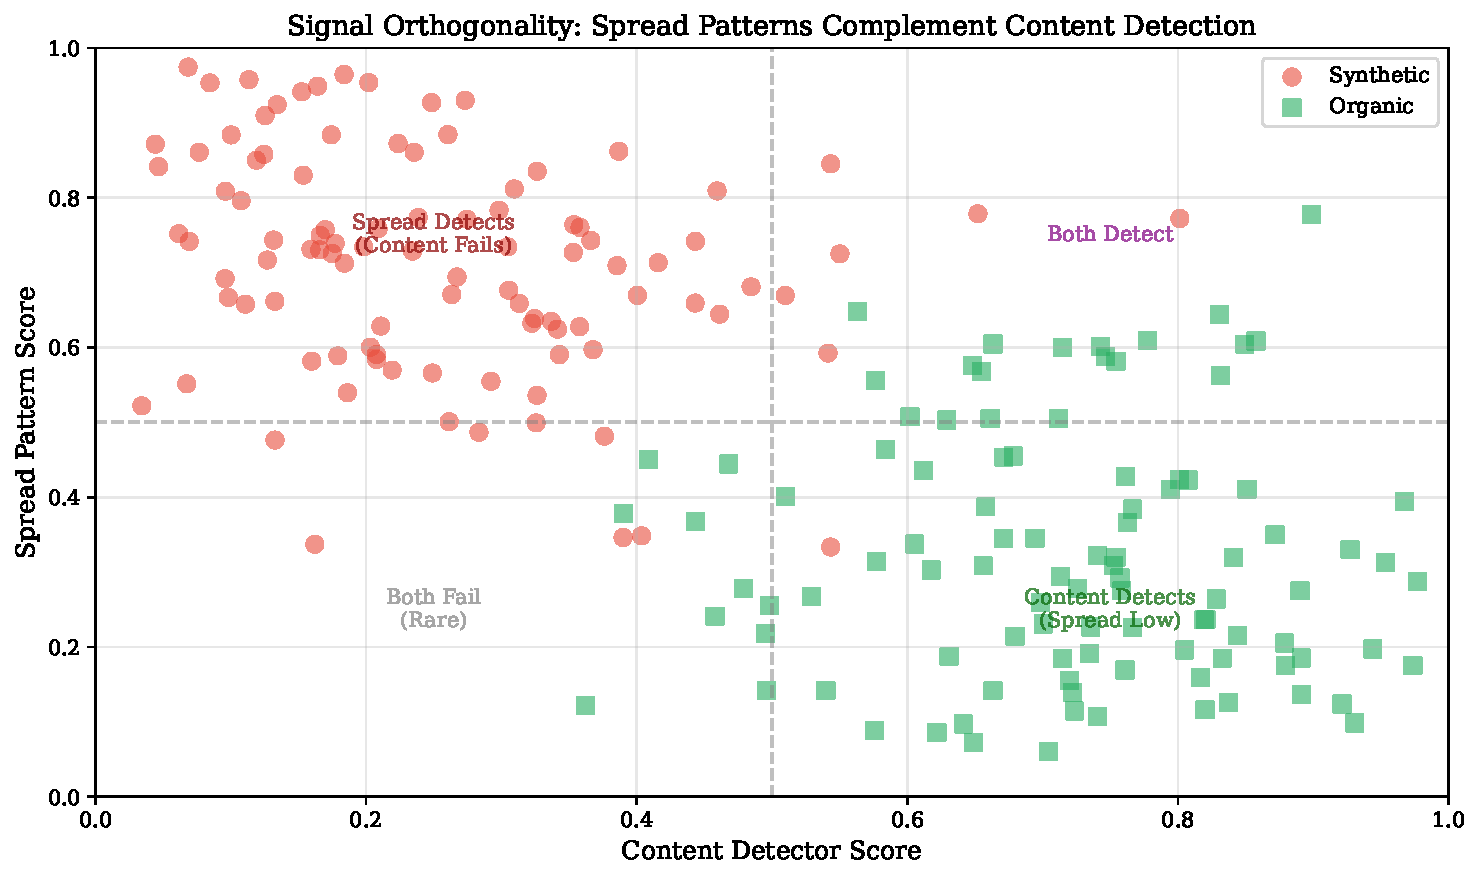
\includegraphics[width=0.8\textwidth]{orthogonality_analysis}
    \caption{Signal orthogonality between content and spread pattern detection. Upper-left quadrant shows cases where spread patterns detect synthetic content that content analysis misses.}
    \label{fig:orthogonality}
\end{figure}

% Figure 5: Statistical Significance
\begin{figure}[htbp]
    \centering
    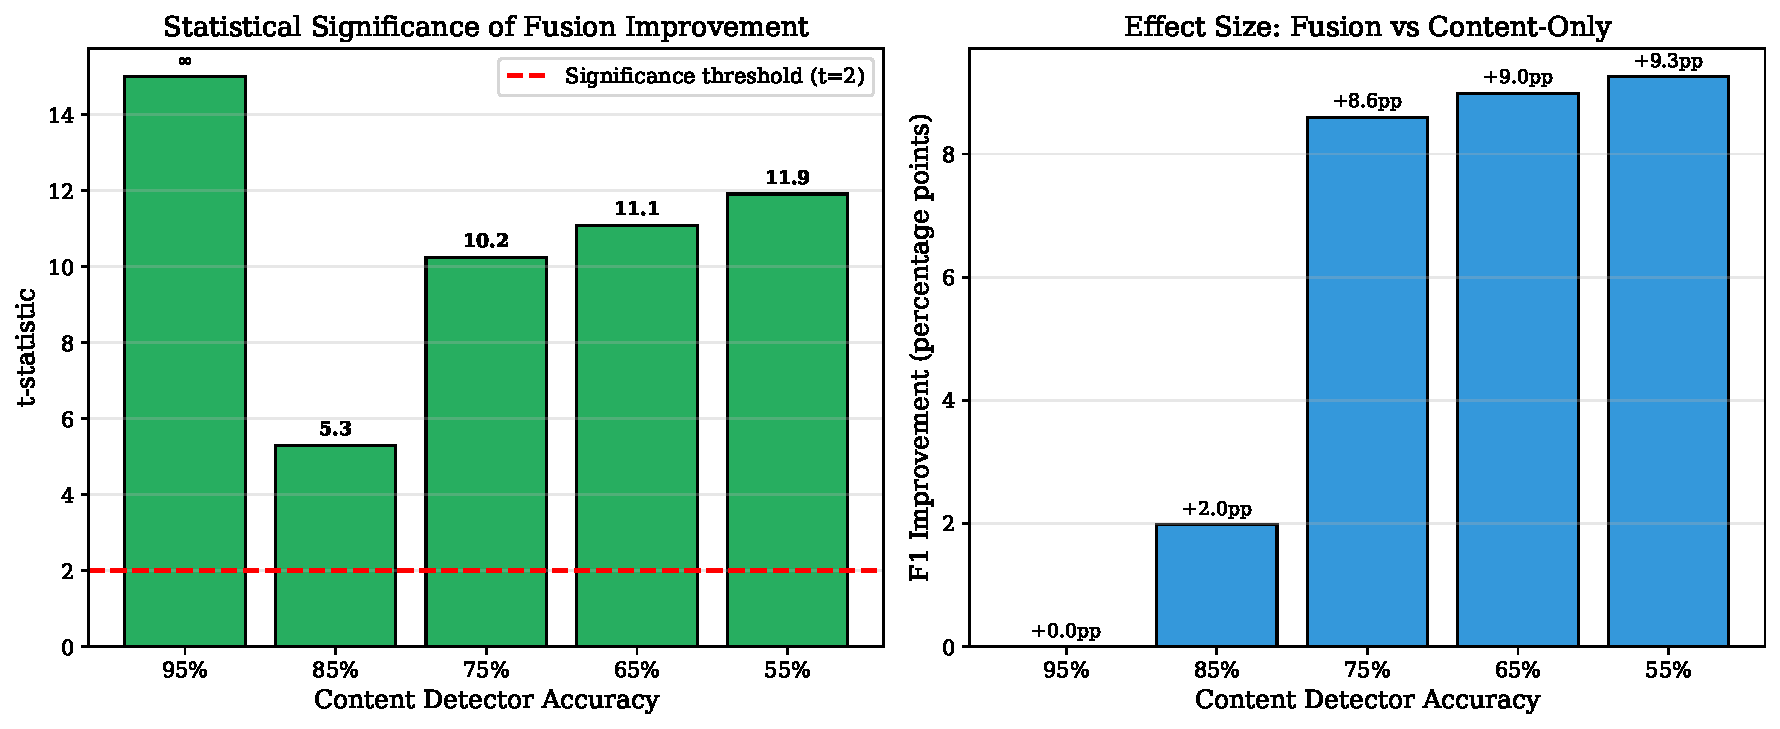
\includegraphics[width=\textwidth]{statistical_significance}
    \caption{Statistical significance of fusion improvements. Left: t-statistics for combined vs content-only comparison (green bars exceed significance threshold). Right: Effect size in percentage points, showing improvements increase as content detector degrades.}
    \label{fig:statistical-significance}
\end{figure}

% Figure 6: Fusion Weight Analysis
\begin{figure}[htbp]
    \centering
    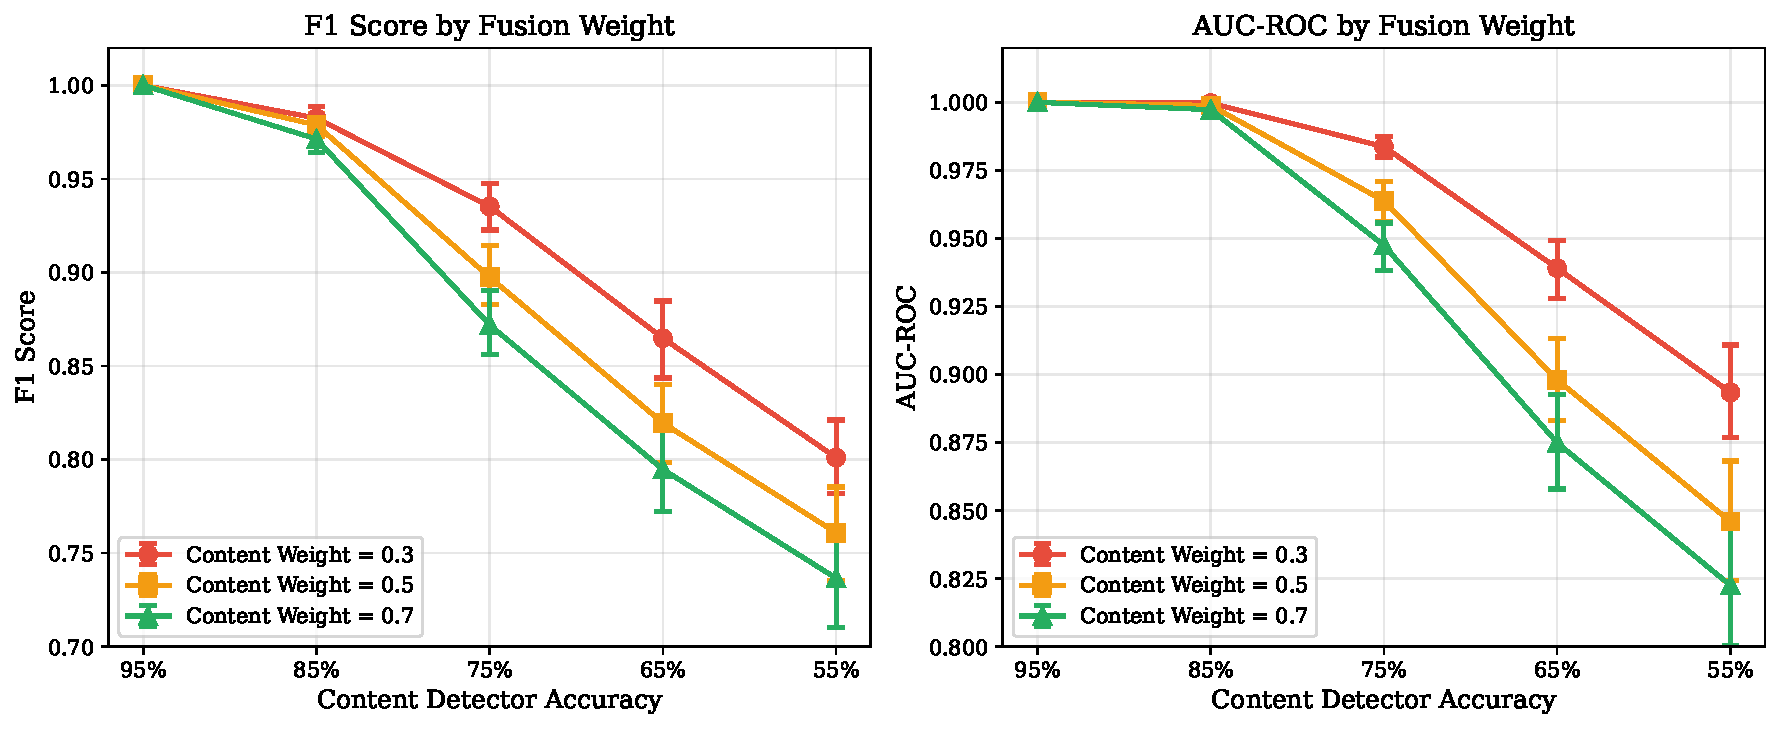
\includegraphics[width=\textwidth]{fusion_weight_analysis}
    \caption{Performance comparison across different fusion weights with 95\% confidence intervals. Lower content weights (more reliance on spread patterns) outperform when content detector accuracy degrades.}
    \label{fig:fusion-weights}
\end{figure}

% Figure 7: Confidence Intervals
\begin{figure}[htbp]
    \centering
    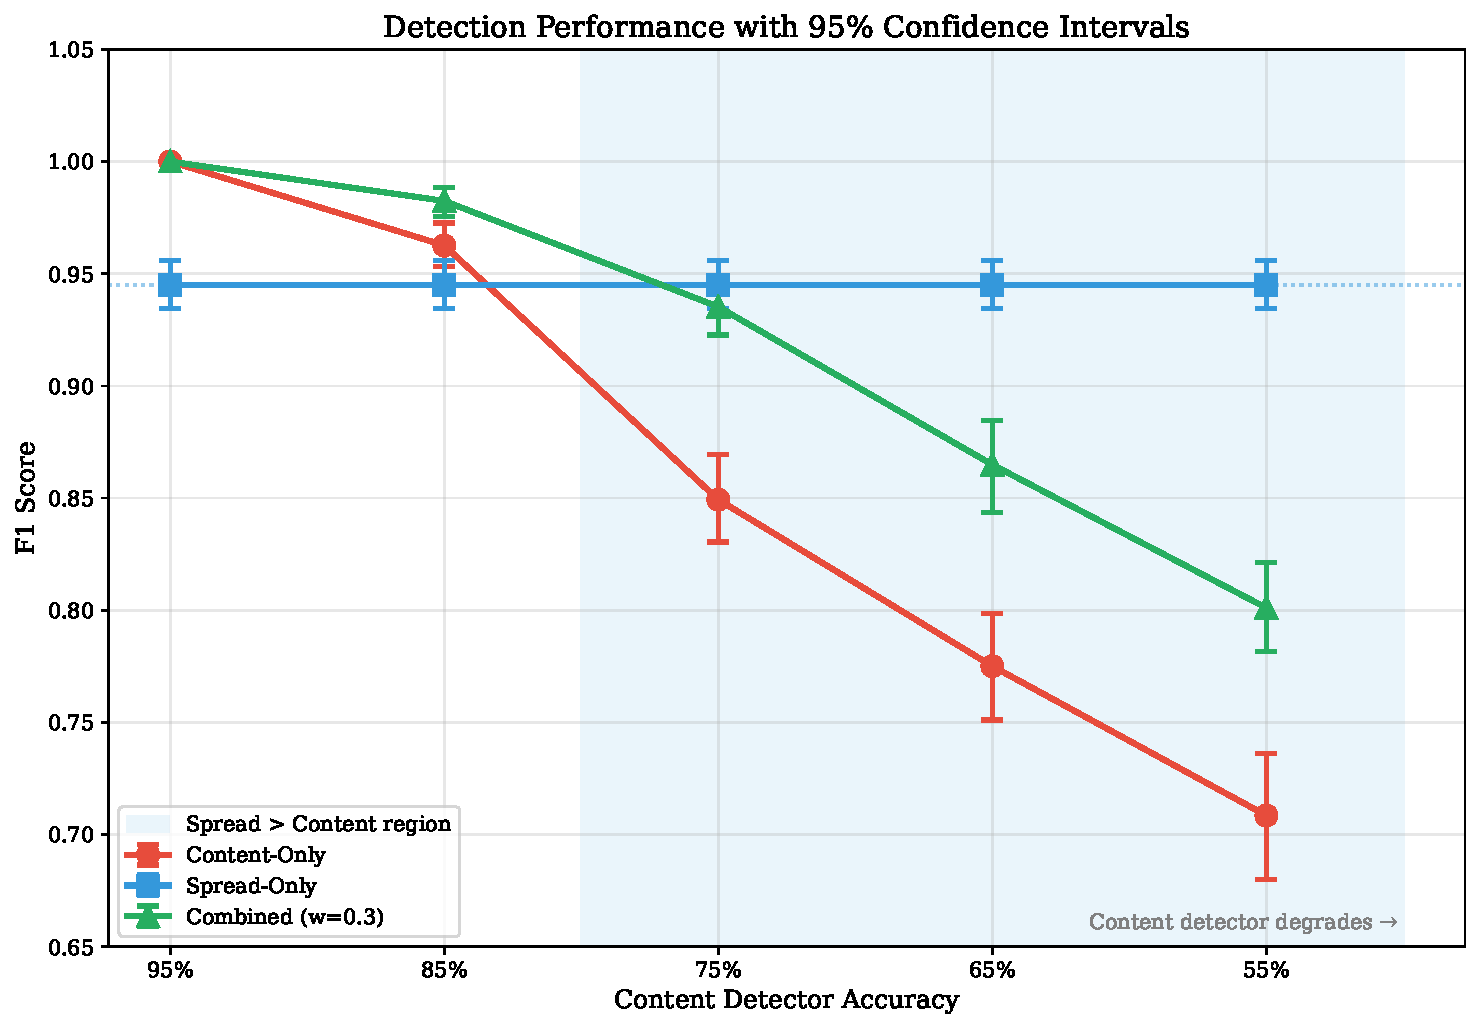
\includegraphics[width=0.9\textwidth]{confidence_intervals}
    \caption{Detection F1 scores with 95\% bootstrap confidence intervals. The shaded region indicates where spread-only detection outperforms content-only. Combined detection maintains robust performance across all conditions.}
    \label{fig:confidence-intervals}
\end{figure}
